\documentclass[11pt,a4paper]{article}
\usepackage{fontspec}
\usepackage[polish]{babel}
\usepackage[margin=2.2cm]{geometry}
\usepackage{graphicx}
\usepackage[table]{xcolor}
\usepackage{listings}
\usepackage{tikz}
\usetikzlibrary{arrows.meta}
\usepackage{amsmath}
\usepackage{booktabs}
\usepackage{caption}
\usepackage{float}
\usepackage{enumitem}
\usepackage{fancyhdr}
\usepackage[hidelinks]{hyperref}

\definecolor{pwr}{HTML}{A4161A}
\definecolor{kod}{HTML}{F6F6F6}

\lstset{
  language=VHDL,
  basicstyle=\ttfamily\small,
  keywordstyle=\color{pwr}\bfseries,
  commentstyle=\color{gray}\itshape,
  backgroundcolor=\color{kod},
  frame=single, rulecolor=\color{gray!40},
  numbers=left, numberstyle=\tiny\color{gray},
  breaklines=true, columns=fullflexible, keepspaces=true,
  xleftmargin=1.5em, framexleftmargin=1.5em
}

\captionsetup{font=small,labelfont=bf}
\setlength{\parindent}{0pt}
\setlength{\parskip}{0.6em}
\setlength{\headheight}{14pt}

\pagestyle{fancy}
\fancyhf{}
\lhead{\small UCiSW 1, laboratorium 2}
\rhead{\small Korwin, Kasiarz}
\cfoot{\thepage}

\newcommand{\nq}[1]{\overline{Q}_{#1}}
\newcommand{\nU}{\overline{U}}
\newcommand{\jj}{\cellcolor{pwr!18}1}

% mapa Karnaugha: wiersze U Q2 = 00, 01, 11, 10; kolumny Q1Q0 = 00, 01, 11, 10
\newcommand{\kmap}[5]{%
  \begin{tabular}{c|cccc}
    \multicolumn{5}{c}{\textbf{#1}}\\[2pt]
    $U\,Q_2 \backslash Q_1Q_0$ & 00 & 01 & 11 & 10\\ \hline
    00 & #2\\
    01 & #3\\
    11 & #4\\
    10 & #5
  \end{tabular}}

\begin{document}

% ---------------- strona tytulowa ----------------
\begin{titlepage}
\centering

\includegraphics[width=3.2cm]{img/pwr_logo.png}\par\vspace{0.8cm}
{\Large\bfseries Politechnika Wrocławska}\par\vspace{2.5cm}
{\large Układy Cyfrowe i Systemy Wbudowane 1}\par\vspace{0.3cm}
{\large Laboratorium}\par\vspace{1.2cm}
{\color{pwr}\rule{0.6\textwidth}{0.8pt}}\par\vspace{0.5cm}
{\LARGE\bfseries Sprawozdanie z laboratorium 2}\par\vspace{0.4cm}
{\Large Trzybitowy licznik rewersyjny}\par\vspace{0.2cm}
{\large wariant b): cykl $0 \to 1 \to 5 \to 2 \to 3 \to 4 \to 6 \to 7$}\par\vspace{0.5cm}
{\color{pwr}\rule{0.6\textwidth}{0.8pt}}\par
\vfill
\begin{tabular}{ll}
\textbf{Wykonali:} & Adam Korwin, 284455\\
                   & Dawid Kasiarz, 284541\\[6pt]
\textbf{Prowadzący:} & dr inż. Jarosław Sugier\\[6pt]
\textbf{Data zajęć:} & 05.11.2026
\end{tabular}
\vspace{1.5cm}
\end{titlepage}

% ---------------- tresc ----------------
\section{Treść zadania}

Celem ćwiczenia było zaprojektowanie trzybitowego licznika rewersyjnego, który w wariancie b) liczy w górę w kolejności $0, 1, 5, 2, 3, 4, 6, 7$, a w dół tą samą drogą w przeciwną stronę. Licznik ma wejście kierunku \texttt{UPnDN} (1 oznacza liczenie w górę), standardowe wejście zezwolenia \texttt{CE}, reset \texttt{Rst} oraz trzybitowe wyjście \texttt{Q(2 downto 0)}. Ćwiczenie składało się z trzech zadań:

\begin{description}[leftmargin=2.2em,style=sameline]
  \item[Z1] opis licznika w VHDL przy pomocy trzech przerzutników typu D z biblioteki UNISIM i zminimalizowanych równań ich wzbudzeń, symulacja behawioralna z zegarem $f_{CLK} = 33\tfrac{1}{3}$~MHz obejmująca pełne cykle w obu kierunkach, a następnie implementacja jako diagram blokowy: zegar 100~MHz z bloku \emph{Clocking Wizard}, dzielnik do 1~Hz (moduł \texttt{ClockDivider}), licznik; $Q$ na diodach LED(2:0), \texttt{CE} z przełącznika SW0, \texttt{UPnDN} z SW1, \texttt{Rst} z przycisku PB3, zegar 1~Hz na diodzie LED7;
  \item[Z2] zastąpienie równań wzbudzeń tabelą zapisaną instrukcją \texttt{with \dots\ select}, do pokazania tylko symulacja behawioralna;
  \item[Z3] licznik taktowany bezpośrednio zegarem 100~MHz (bez dzielnika) i przełączany obrotami enkodera (moduł \texttt{RotaryEnc}): impulsy \texttt{RotL} i \texttt{RotR} wytwarzają sygnały \texttt{CE} oraz \texttt{UPnDN}.
\end{description}

\section{Z1: projekt licznika}

\subsection{Tabela przejść}

Przerzutnik D przy narastającym zboczu zegara przepisuje wejście $D$ na wyjście $Q$. Wzbudzenie każdego przerzutnika jest więc po prostu odpowiednim bitem stanu następnego. Pełną tabelę przejść dla obu kierunków zawiera tabela~\ref{tab:przejscia}. Oznaczyliśmy $U = \texttt{UPnDN}$.

\begin{table}[H]
\centering
\small
\begin{tabular}{ccc@{\hspace{3em}}ccc}
\toprule
\multicolumn{3}{c}{w górę ($U = 1$)} & \multicolumn{3}{c}{w dół ($U = 0$)}\\
\cmidrule(r{2em}){1-3}\cmidrule{4-6}
$Q$ & $Q_2Q_1Q_0$ & $D_2D_1D_0$ & $Q$ & $Q_2Q_1Q_0$ & $D_2D_1D_0$\\
\midrule
0 & 000 & 001 (1) & 0 & 000 & 111 (7)\\
1 & 001 & 101 (5) & 1 & 001 & 000 (0)\\
2 & 010 & 011 (3) & 2 & 010 & 101 (5)\\
3 & 011 & 100 (4) & 3 & 011 & 010 (2)\\
4 & 100 & 110 (6) & 4 & 100 & 011 (3)\\
5 & 101 & 010 (2) & 5 & 101 & 001 (1)\\
6 & 110 & 111 (7) & 6 & 110 & 100 (4)\\
7 & 111 & 000 (0) & 7 & 111 & 110 (6)\\
\bottomrule
\end{tabular}
\caption{Tabela przejść licznika. W nawiasach stan następny dziesiętnie.}
\label{tab:przejscia}
\end{table}

\subsection{Wybór przerzutnika}

W rodzinie Zynq UltraScale+ podstawowym przerzutnikiem typu D w bibliotece UNISIM jest \texttt{FDRE}. Ma on wejście danych \texttt{D}, zegar \texttt{C}, zezwolenie \texttt{CE} oraz synchroniczny reset \texttt{R} do zera. Sygnały \texttt{CE} i \texttt{Rst} licznika podłączyliśmy bezpośrednio do tych wejść, więc obsługuje je sam przerzutnik. Dzięki temu równania wzbudzeń zależą tylko od czterech zmiennych: $U$, $Q_2$, $Q_1$, $Q_0$, i każde z nich można zminimalizować na mapie Karnaugha $4 \times 4$.

\subsection{Minimalizacja w tablicach Karnaugha}

W mapach wiersze opisują $U Q_2$, a kolumny $Q_1Q_0$, obie osie w kodzie Graya. Dwa górne wiersze ($U = 0$) odpowiadają liczeniu w dół, dwa dolne ($U = 1$) liczeniu w górę. Pola z jedynkami są wyróżnione kolorem.

\begin{figure}[H]
\centering
\small
\kmap{$D_2$}{\jj&0&0&\jj}{0&0&\jj&\jj}{\jj&0&0&\jj}{0&\jj&\jj&0}
\hspace{1.5em}
\kmap{$D_1$}{\jj&0&\jj&0}{\jj&0&\jj&0}{\jj&\jj&0&\jj}{0&0&0&\jj}
\\[1.2em]
\kmap{$D_0$}{\jj&0&0&\jj}{\jj&\jj&0&0}{0&0&0&\jj}{\jj&\jj&0&\jj}
\caption{Tablice Karnaugha dla wzbudzeń przerzutników.}
\end{figure}

Odczytane grupy:

\textbf{$D_2$.} W wierszu 00 jedynki leżą w skrajnych kolumnach, które są sąsiednie, co daje $\nU\nq{2}\nq{0}$ ($Q = 0, 2$ przy liczeniu w dół). W wierszu 01 kolumny 11 i 10 dają $\nU Q_2 Q_1$ ($Q = 7, 6$). Przy liczeniu w górę mamy $U\nq{2}Q_0$ (wiersz 10, $Q = 1, 3$) oraz $U Q_2 \nq{0}$ (wiersz 11, skrajne kolumny, $Q = 4, 6$).

\textbf{$D_1$.} Kolumny 00 i 11 w dwóch górnych wierszach dają $\nU\nq{1}\nq{0}$ ($Q = 0, 4$) i $\nU Q_1 Q_0$ ($Q = 3, 7$). W dolnej połowie mapy pozostają $U Q_2 \nq{1}$ ($Q = 4, 5$) oraz $U Q_1 \nq{0}$ (kolumna 10 w wierszach 11 i 10, $Q = 6, 2$).

\textbf{$D_0$.} Wiersz 01, kolumny 00 i 01 dają $\nU Q_2 \nq{1}$ ($Q = 4, 5$). Wiersz 10, te same kolumny, daje $U \nq{2} \nq{1}$ ($Q = 0, 1$). Kolumna 10 w dolnych wierszach to $U Q_1 \nq{0}$ ($Q = 6, 2$). Ostatnia grupa, $\nq{2}\nq{0}$, łączy narożniki wierszy 00 i 10, czyli stany 0 i 2 niezależnie od kierunku, bo skrajne wiersze i kolumny mapy są sąsiednie.

Otrzymane równania:
\begin{align*}
D_2 &= \nU\nq{2}\nq{0} + \nU Q_2 Q_1 + U\nq{2}Q_0 + U Q_2\nq{0}\\
D_1 &= \nU\nq{1}\nq{0} + \nU Q_1 Q_0 + U Q_2\nq{1} + U Q_1\nq{0}\\
D_0 &= \nU Q_2\nq{1} + U\nq{2}\nq{1} + U Q_1\nq{0} + \nq{2}\nq{0}
\end{align*}

Warto zauważyć, że dla $U = 1$ wzbudzenie $D_2$ upraszcza się do $Q_2 \oplus Q_0$, a dla $U = 0$ wzbudzenie $D_1$ do $\overline{Q_1 \oplus Q_0}$. Poprawność równań sprawdziliśmy krótkim skryptem w Pythonie, który porównuje wynik równań z tabelą~\ref{tab:przejscia} dla wszystkich szesnastu kombinacji $(U, Q)$.

\subsection{Opis w VHDL}

Równania zapisaliśmy jako przypisania współbieżne do sygnału pomocniczego \texttt{D}, a trzy przerzutniki \texttt{FDRE} wstawiliśmy jako instancje komponentu z biblioteki UNISIM. Wyjścia przerzutników są dostępne wewnątrz architektury jako sygnał \texttt{Qi}, ponieważ w VHDL-93 nie można odczytywać portu wyjściowego \texttt{Q}. Przy mieszaniu operatorów \texttt{and} i \texttt{or} każdy iloczyn jest ujęty w nawiasy.

\lstinputlisting[caption={Plik \texttt{Licznik\_b.vhd}}]{../Licznik_b.vhd}

\subsection{Testbench i wynik symulacji}

Zegar o częstotliwości $33\tfrac{1}{3}$~MHz ma okres 30~ns, więc w testbenchu sygnał \texttt{Clk} zmienia stan co 15~ns, a zbocza narastające wypadają w chwilach 15, 45, 75, \dots~ns. Pozostałe wymuszenia zmieniają się pomiędzy zboczami narastającymi. Przebieg testu:
\begin{itemize}[itemsep=0pt]
  \item 0--60~ns: reset aktywny, licznik w stanie 0;
  \item 60--300~ns: osiem taktów w górę, pełny cykl $0, 1, 5, 2, 3, 4, 6, 7, 0$;
  \item 300--540~ns: osiem taktów w dół, pełny cykl $0, 7, 6, 4, 3, 2, 5, 1, 0$;
  \item 540--600~ns: \texttt{CE} = 0, licznik stoi;
  \item 600--690~ns: znów w górę ($1, 5, 2$), następnie reset w trakcie liczenia, po którym licznik startuje od zera.
\end{itemize}

Proces \texttt{Check} liczy równolegle model licznika na podstawie tabeli przejść i 10~ns po każdym zboczu porównuje go z wyjściem $Q$. W razie niezgodności wypisuje komunikat \texttt{Blad: Q = ..., oczekiwano ...}.

\lstinputlisting[caption={Plik \texttt{Licznik\_tb.vhd}}]{../Licznik_tb.vhd}

Symulacja zakończyła się komunikatem \texttt{Koniec testu} w chwili 805~ns i nie pojawił się żaden komunikat o błędzie. Przebieg z symulatora Vivado przedstawia rysunek~\ref{fig:sim_foto}, a uporządkowany schemat tych samych przebiegów rysunek~\ref{fig:sim}.

\begin{figure}[H]
\centering
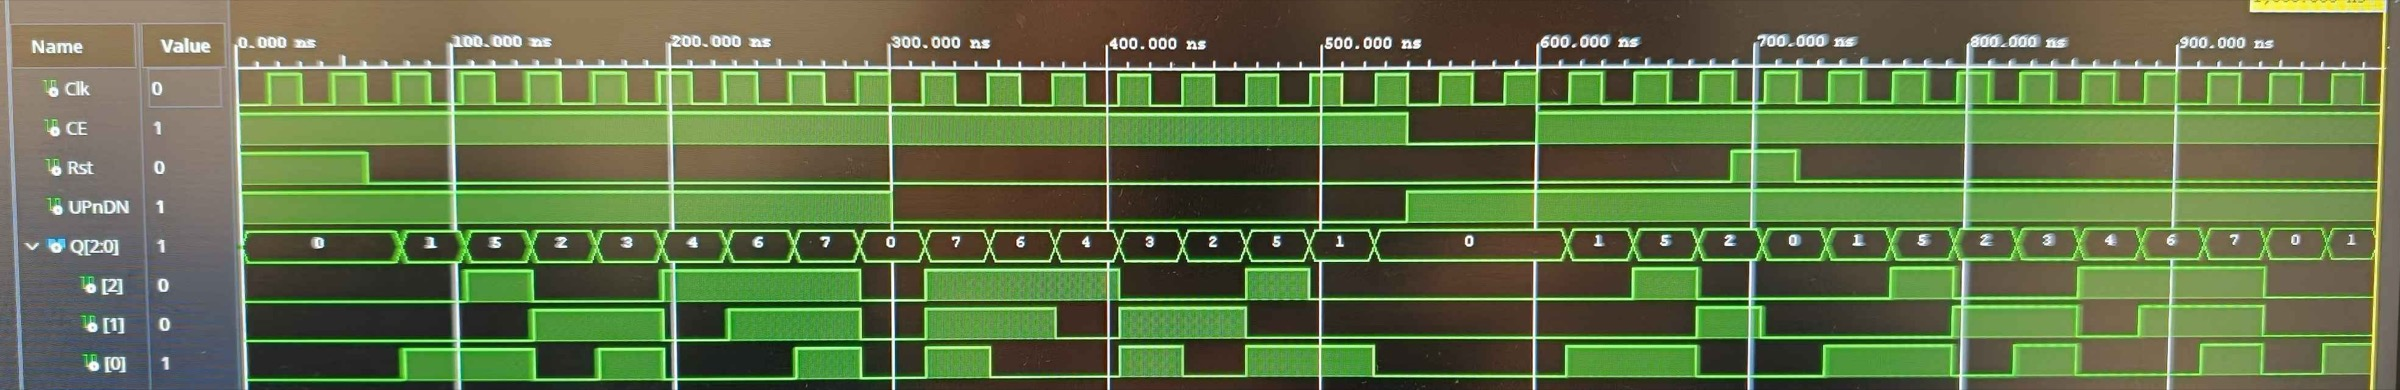
\includegraphics[width=\textwidth]{img/sim_z1.jpg}
\caption{Symulacja behawioralna w Vivado (zdjęcie ekranu z zajęć). Szyna \texttt{Q[2:0]} jest pokazana dziesiętnie, pod nią bity $Q(2)$, $Q(1)$, $Q(0)$.}
\label{fig:sim_foto}
\end{figure}

\begin{figure}[H]
\centering
\begin{tikzpicture}[x=0.0178cm,y=1cm,font=\scriptsize]
  % podswietlenie: cykl w gore i w dol
  \fill[pwr!8]  (75,-0.45) rectangle (315,4.45);
  \fill[gray!12] (315,-0.45) rectangle (555,4.45);
  \node[anchor=east] at (-5,4) {\texttt{Clk}};
  \node[anchor=east] at (-5,3) {\texttt{Rst}};
  \node[anchor=east] at (-5,2) {\texttt{CE}};
  \node[anchor=east] at (-5,1) {\texttt{UPnDN}};
  \node[anchor=east] at (-5,0) {\texttt{Q}};
  % zegar
  \foreach \t in {0,30,...,780} {
    \draw (\t,3.75) -- (\t+15,3.75) -- (\t+15,4.25) -- (\t+30,4.25) -- (\t+30,3.75);
  }
  % sygnaly sterujace
  \draw (0,3.25) -- (60,3.25) -- (60,2.75) -- (690,2.75) -- (690,3.25) -- (720,3.25) -- (720,2.75) -- (810,2.75);
  \draw (0,2.25) -- (540,2.25) -- (540,1.75) -- (600,1.75) -- (600,2.25) -- (810,2.25);
  \draw (0,1.25) -- (300,1.25) -- (300,0.75) -- (540,0.75) -- (540,1.25) -- (810,1.25);
  % szyna Q
  \foreach \a/\b/\v in {0/75/0,75/105/1,105/135/5,135/165/2,165/195/3,195/225/4,225/255/6,255/285/7,
                        285/315/0,315/345/7,345/375/6,375/405/4,405/435/3,435/465/2,465/495/5,495/525/1,
                        525/615/0,615/645/1,645/675/5,675/705/2,705/735/0,735/765/1,765/795/5,795/810/2} {
    \draw (\a,0) -- (\a+3,0.25) -- (\b-3,0.25) -- (\b,0) -- (\b-3,-0.25) -- (\a+3,-0.25) -- cycle;
    \node at ({(\a+\b)/2},0) {\v};
  }
  % os czasu
  \draw[gray] (0,-0.65) -- (810,-0.65);
  \foreach \t in {0,100,...,800} {
    \draw[gray] (\t,-0.65) -- (\t,-0.75);
    \node[gray,below] at (\t,-0.75) {\t};
  }
  \node[pwr] at (195,4.65) {w górę};
  \node[gray!70!black] at (435,4.65) {w dół};
\end{tikzpicture}
\caption{Przebiegi z symulacji behawioralnej, oś czasu w ns. Kolorem zaznaczono pełny cykl w górę (75--315~ns) i pełny cykl w dół (315--555~ns).}
\label{fig:sim}
\end{figure}

\subsection{Implementacja jako diagram blokowy}

W tym samym projekcie utworzyliśmy diagram blokowy (\emph{IP Integrator}) i dodaliśmy do niego moduły RTL \texttt{Licznik} oraz \texttt{ClockDivider}, który otrzymaliśmy od prowadzącego. Dzielnik zlicza takty zegara wejściowego i co $\frac{f_{IN}}{2 f_{OUT}}$ taktów zmienia stan wyjścia, a parametry \texttt{IN\_FREQ\_HZ} = 100E6 i \texttt{OUT\_FREQ\_HZ} = 1 dają zegar 1~Hz. Zegar 100~MHz dostarcza blok \emph{Clocking Wizard} podłączony do różnicowego zegara płyty (\emph{Board}, \emph{Differential Clock}, \emph{Auto Connect}), z którego usunęliśmy niepotrzebne wejście \texttt{reset} i wyjście \texttt{locked}. Strukturę diagramu przedstawia rysunek~\ref{fig:bd_z1}.

\begin{figure}[H]
\centering
\begin{tikzpicture}[font=\small,
  blk/.style={draw,fill=pwr!10,rounded corners=2pt,minimum height=1.4cm,minimum width=2.6cm,align=center},
  port/.style={draw,fill=gray!15,font=\ttfamily\footnotesize,inner sep=2pt},
  >={Stealth[length=2mm]}]
  \node[blk] (wiz) at (0,0) {\texttt{clk\_wiz\_0}\\[-1pt]\scriptsize Clocking Wizard};
  \node[blk] (div) at (4.2,0) {\texttt{ClockDivider\_0}\\[-1pt]\scriptsize 100 MHz $\to$ 1 Hz};
  \node[blk,minimum height=2.4cm,minimum width=3cm,label={[font=\ttfamily\small]above:Licznik\_0}] (lic) at (9.2,-0.5) {};
  \node[port,anchor=east] (clk) at (-2.0,0) {clk\_100mhz};
  \node[port,anchor=east] (ce)  at (6.4,-0.7) {CE};
  \node[port,anchor=east] (ud)  at (6.4,-1.2) {UPnDN};
  \node[port,anchor=east] (rst) at (6.4,-1.7) {Rst};
  \node[port,anchor=west] (q)   at (11.2,-0.5) {Q[2:0]};
  \node[port,anchor=west] (c1)  at (11.2,1.6) {Clk\_1Hz};
  \draw[->] (clk) -- (wiz);
  \draw[->] (wiz) -- node[above,font=\scriptsize]{100 MHz} (div);
  \draw[->] (div.east) -- (6.9,0) |- (c1);
  \draw[->] (6.9,0) -- (7.7,0) node[right,font=\scriptsize]{Clk};
  \draw[->] (ce)  -- (7.7,-0.7)  node[right,font=\scriptsize]{CE};
  \draw[->] (ud)  -- (7.7,-1.2)  node[right,font=\scriptsize]{UPnDN};
  \draw[->] (rst) -- (7.7,-1.7)  node[right,font=\scriptsize]{Rst};
  \draw[->] (lic) -- (q);
  \fill (6.9,0) circle (1.5pt);
\end{tikzpicture}
\caption{Schemat diagramu blokowego zadania Z1.}
\label{fig:bd_z1}
\end{figure}

Porty zewnętrzne utworzyliśmy poleceniem \emph{Create Port}, nadając im od razu nazwy zgodne z plikiem ograniczeń. Numery wyprowadzeń przepisaliśmy z pliku \texttt{ZU3.xdc} udostępnionego przez prowadzącego. Linii zegara w pliku XDC nie ma, ponieważ opisuje go \emph{Clocking Wizard}.

\lstinputlisting[language={},caption={Plik \texttt{Z1.xdc}}]{../Z1.xdc}

Po walidacji diagramu, utworzeniu pliku \emph{HDL Wrapper} i wygenerowaniu pliku \texttt{.bit} zaprogramowaliśmy układ przez Hardware Manager. Działanie sprawdziliśmy według tabeli~\ref{tab:plyta}. Dioda LD7 migała z częstotliwością 1~Hz, a stan licznika zmieniał się na każdym jej zapaleniu.

\begin{table}[H]
\centering
\small
\begin{tabular}{cccl}
\toprule
SW1 (\texttt{UPnDN}) & SW0 (\texttt{CE}) & PB3 (\texttt{Rst}) & LD2 LD1 LD0 (co sekundę)\\
\midrule
1 & 1 & -- & $0, 1, 5, 2, 3, 4, 6, 7, 0, \dots$\\
0 & 1 & -- & $0, 7, 6, 4, 3, 2, 5, 1, 0, \dots$\\
x & 0 & -- & stan nie zmienia się\\
x & x & wciśnięty & 000\\
\bottomrule
\end{tabular}
\caption{Test licznika na płycie.}
\label{tab:plyta}
\end{table}

\section{Z2: wzbudzenia zapisane tabelą}

W drugiej wersji licznika zamiast równań wpisaliśmy wprost tabelę przejść. Kierunek i stan bieżący sklejamy w czterobitowy wektor \texttt{Sel = UPnDN \& Qi}, a instrukcja \texttt{with Sel select} przypisuje każdej z szesnastu wartości odpowiednie wzbudzenie $D$. Sygnał pośredni \texttt{Sel} jest potrzebny, ponieważ w VHDL-93 wyrażeniem wyboru nie może być konkatenacja. Gałąź \texttt{when others} jest wymagana, bo typ \texttt{std\_logic} ma oprócz 0 i 1 także wartości \texttt{U}, \texttt{X}, \texttt{Z} i inne. Przerzutniki, encja i porty pozostały bez zmian. Wersję tabelaryczną umieściliśmy w osobnym projekcie, ponieważ obie wersje definiują encję o tej samej nazwie \texttt{Licznik}.

\lstinputlisting[caption={Plik \texttt{Licznik\_b\_tab.vhd}}]{../Licznik_b_tab.vhd}

Do symulacji użyliśmy tego samego testbencha co w Z1. Przebiegi były identyczne jak na rysunku~\ref{fig:sim}, a symulacja zakończyła się komunikatem \texttt{Koniec testu} bez komunikatów o błędach. Dodatkowo, aby upewnić się, że proces \texttt{Check} rzeczywiście wykrywa błędy, zmieniliśmy na próbę jeden wiersz tabeli (przejście $5 \to 2$ zamieniliśmy na $5 \to 3$). W takiej symulacji pojawiły się komunikaty \texttt{Blad}, co potwierdza, że test sprawdza wynik, a nie tylko dochodzi do końca.

Obie wersje opisują tę samą funkcję czterech zmiennych dla każdego bitu $D$, więc po syntezie każde wzbudzenie zajmuje jedną tablicę LUT niezależnie od sposobu zapisu. Zapis tabelaryczny nie wymaga minimalizacji i jest łatwiejszy do sprawdzenia, natomiast równania pokazują strukturę logiki.

\section{Z3: licznik sterowany enkoderem}

Projekt z Z1 zapisaliśmy pod nową nazwą (\emph{Save Project As}) i zmodyfikowaliśmy diagram. Usunęliśmy dzielnik zegara oraz porty \texttt{CE}, \texttt{UPnDN} i \texttt{Clk\_1Hz}, a dodaliśmy moduł \texttt{RotaryEnc} od prowadzącego oraz blok IP \emph{Utility Vector Logic} skonfigurowany jako jednobitowa bramka OR (\texttt{C\_SIZE} = 1, \texttt{C\_OPERATION} = or). Licznik i enkoder pracują teraz z zegarem 100~MHz.

Moduł \texttt{RotaryEnc} synchronizuje sygnały \texttt{ROT\_A} i \texttt{ROT\_B} enkodera z zegarem i przy każdym „kliknięciu” pokrętła wytwarza na wyjściu \texttt{RotR} (obrót w prawo) lub \texttt{RotL} (obrót w lewo) impuls trwający dokładnie jeden takt zegara. Sygnały licznika powstają następująco:
\begin{itemize}[itemsep=0pt]
  \item \texttt{CE = RotL or RotR}: licznik wykonuje krok tylko w takcie, w którym pojawił się impuls, czyli jeden krok na jedno kliknięcie;
  \item \texttt{UPnDN = RotR}: podczas impulsu \texttt{RotR} kierunek wynosi 1 (w górę), podczas impulsu \texttt{RotL} wynosi 0 (w dół). Poza impulsami wartość \texttt{UPnDN} nie ma znaczenia, bo \texttt{CE} = 0.
\end{itemize}

Gotowy diagram przedstawia rysunek~\ref{fig:bd_z3}.

\begin{figure}[H]
\centering
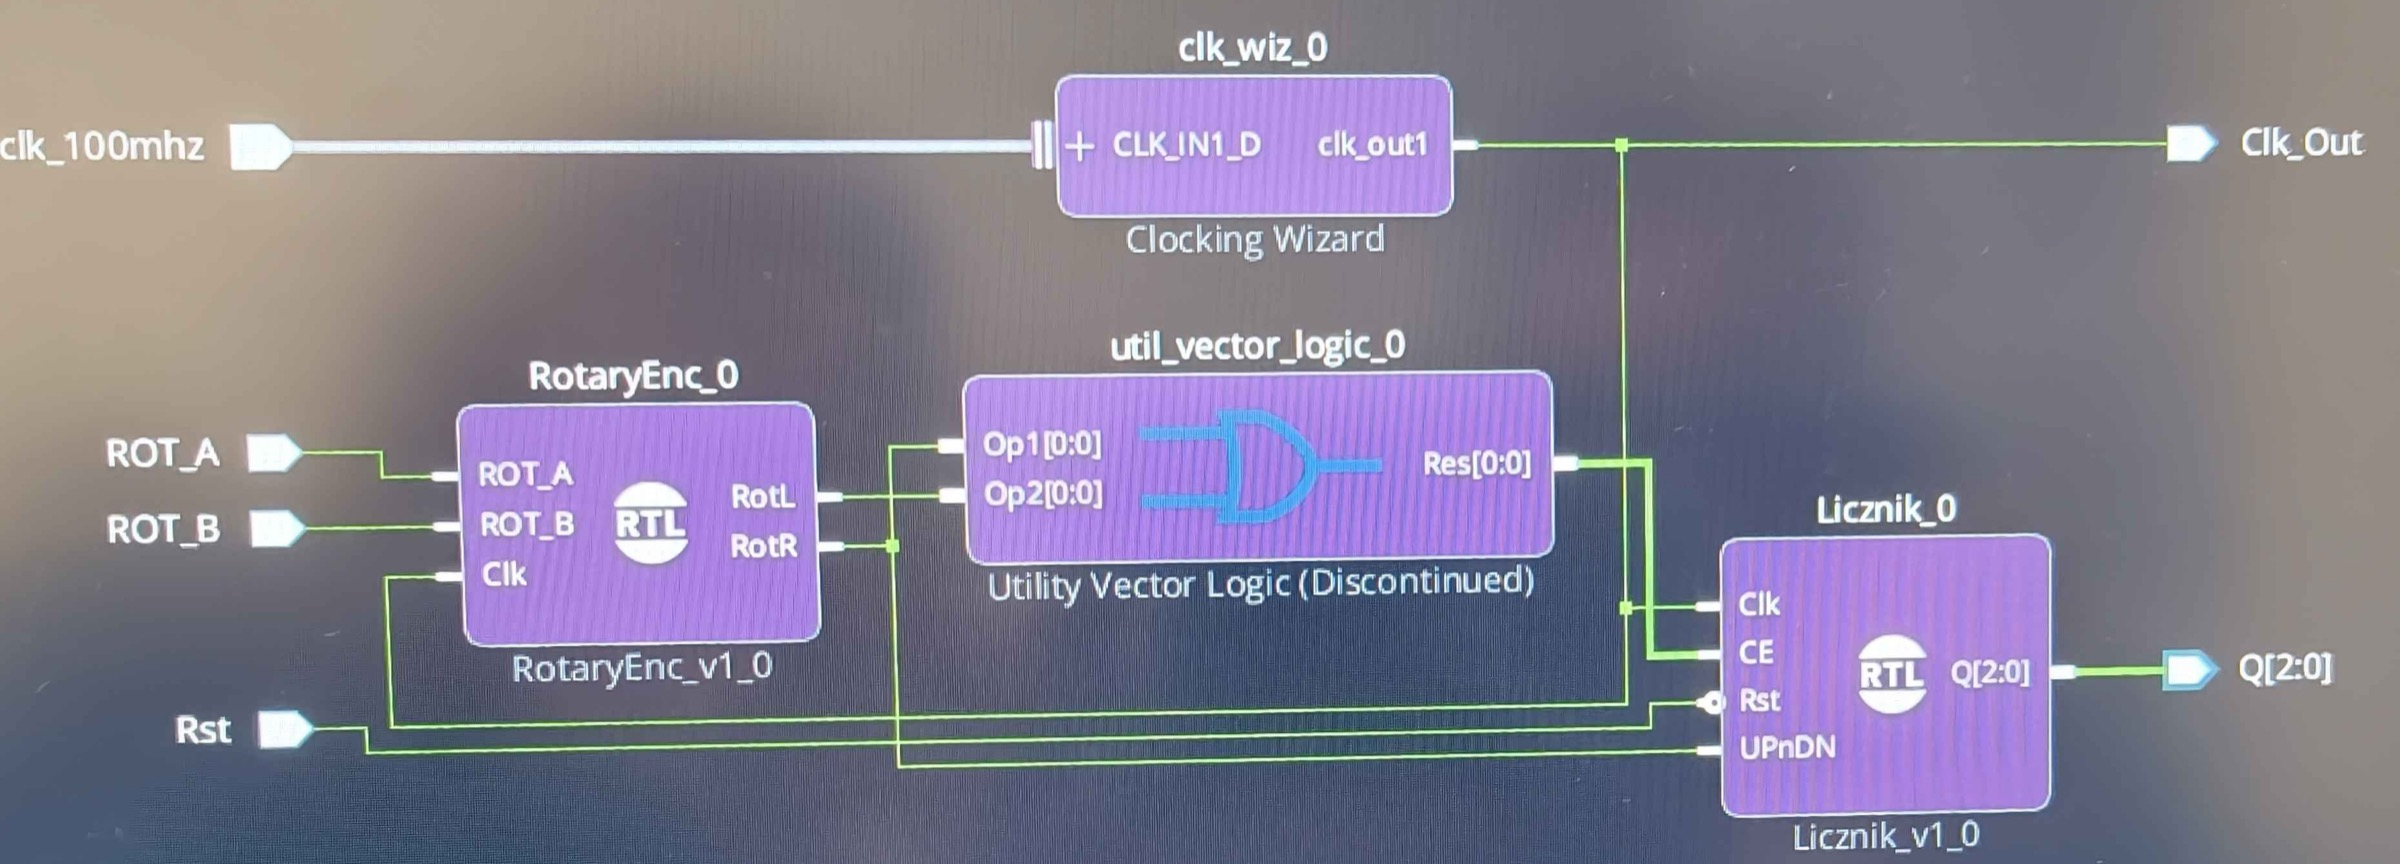
\includegraphics[width=\textwidth]{img/bd_z3.jpg}
\caption{Diagram blokowy zadania Z3 (zdjęcie ekranu z zajęć). Bramka OR (\texttt{util\_vector\_logic\_0}) tworzy \texttt{CE}, a wyjście \texttt{RotR} jest jednocześnie sygnałem \texttt{UPnDN}.}
\label{fig:bd_z3}
\end{figure}

Sygnały enkodera są wyprowadzone na płytę rozszerzającą, która pracuje w standardzie \texttt{LVCMOS33}. Numery wyprowadzeń wzięliśmy z pliku \texttt{ZU3\_Exp.xdc}.

\lstinputlisting[language={},caption={Plik \texttt{Z3.xdc}}]{../Z3.xdc}

Sam licznik jest tym samym modułem, którego poprawność potwierdziły symulacje w Z1 i Z2 oraz test na płycie w Z1. Zmienia się jedynie źródło sygnałów \texttt{CE} i \texttt{UPnDN}. W tym układzie każde kliknięcie pokrętła w prawo przesuwa licznik o jeden stan w górę cyklu, a kliknięcie w lewo o jeden stan w dół. Przycisk PB3 zeruje licznik.

\section{Wnioski}

Użycie przerzutników \texttt{FDRE}, które mają wbudowane wejścia zezwolenia i synchronicznego resetu, znacznie uprościło projekt. Sygnały \texttt{CE} i \texttt{Rst} nie występują w równaniach wzbudzeń, więc każde z nich jest funkcją tylko czterech zmiennych i daje się zminimalizować na zwykłej mapie Karnaugha $4 \times 4$. Symulacja behawioralna potwierdziła poprawność pełnych cykli w obu kierunkach oraz działanie \texttt{CE} i resetu w trakcie liczenia.

Zastąpienie równań tabelą \texttt{with \dots\ select} dało identyczny wynik symulacji. Zapis tabelaryczny jest mniej podatny na pomyłki, bo przepisuje się go wprost z tabeli przejść, a narzędzie syntezy samo wykonuje minimalizację.

W zadaniu Z3 licznik jest taktowany z pełną częstotliwością 100~MHz, a o tym, kiedy wykonuje krok, decyduje wyłącznie sygnał \texttt{CE}. Takie rozwiązanie, w którym jednym zegarem taktowany jest cały układ, a zdarzenia są sygnalizowane jednotaktowymi impulsami zezwolenia, jest bezpieczniejsze niż taktowanie licznika bezpośrednio sygnałem z enkodera lub z dzielnika, ponieważ cała logika pozostaje w jednej domenie zegarowej.

\end{document}
